\documentclass[a4paper]{article}
\usepackage[a4paper, left=5mm, right=5mm, top=5mm, bottom=5mm]{geometry}
%\geometry{paperwidth=210mm, paperheight=2000pt, left=5pt, top=5pt}
\usepackage[utf8]{inputenc}
\usepackage[english,russian]{babel}
\usepackage{indentfirst}
\usepackage{tikz} %Рисование автоматов
\usetikzlibrary{automata,positioning,arrows,trees,calc}
\usepackage{amsmath}
\usepackage[makeroom]{cancel} % зачеркивание
\usepackage{multicol,multirow} %Несколько колонок
\usepackage{hyperref}
\usepackage{tabularx}
\usepackage{amsfonts}
\usepackage{amssymb}
\DeclareMathOperator*{\argmin}{arg\,min}
\usepackage{listings}
\usepackage{wasysym}
\date{задано 2014.04.17}
\author{Сергей~Володин, 272 гр.}
\newcommand{\matrixl}{\left|\left|}
\newcommand{\matrixr}{\right|\right|}
% названия автоматов  (rubtsov)
\def\A{{\cal A}}
\def\B{{\cal B}}
\def\C{{\cal C}}

%классы сложности (rubtsov)
\def\PP{{\mathsf{P}}}
\def\NP{{\mathsf{NP}}}
\def\NPc{{\mathsf{NP}}\text{-}{\rm c}}
\def\coNP{{\rm co}\text{-}{\mathsf{NP}}}
\def\DTIME{{\mathsf{DTIME}}}
\def\NTIME{{\mathsf{NTIME}}}
\def\CLIQUE{{\mathsf{CLIQUE}}}
\def\HALT{{\rm{HALT}}}
\def\SAT{{\rm{SAT}}}
\def\3SAT{{\rm{3\text{-}SAT}}}
\def\2SAT{{\rm{2\text{-}SAT}}}
\def\UNSAT{{\rm{UNSAT}}}
\def\HP{{\rm{HAMPATH}}}
\def\UHP{{\rm{UHAMPATH}}}
\def\LL{{\mathrm{LL}}}
\def\poly{{\rm{poly}}}
\def\GC{{\mbox{ГЦ}}}
\def\GP{{\mbox{ГП}}}
\def\conv{{\mbox{conv}}}

\title{Алгоритмы и модели вычислений.\\Задание 11: DFT}

% алгоритмы (Рубцов)
\usepackage{verbatim}
\usepackage{listings}
\usepackage{algorithm2e}

%+= и -=, иначе разъезжаются...
\newcommand{\peq}{\mathrel{+}=}
\newcommand{\meq}{\mathrel{-}=}
\newcommand{\deq}{\mathrel{:}=}
\newcommand{\plpl}{\mathrel{+}+}

\newcommand{\todo}{{\em todo}}

% пустое слово  (rubtsov)
\def\eps{\varepsilon}

% регулярные языки  (rubtsov)
\def\REG{{\mathsf{REG}}}
\def\CFL{{\mathsf{CFL}}}
\def\eqdef{\overset{\mbox{\tiny def}}{=}}
\newcommand{\niton}{\not\owns}

%FIRST & FOLLOW (rubtsov)
\def\first{\mathrm{ FIRST} }
\def\follow{\mathrm{ FOLLOW} }

% LL LR (rubtsov)
\def\LL{{\mathrm{LL}}}
\def\LR{{\mathrm{LR}}}

\newcounter{rowItemCount}
\newcounter{subRowItemCount}
\newcommand\rowItem{
    \setcounter{subRowItemCount}{0}
    \arabic{rowItemCount}.\addtocounter{rowItemCount}{1}}
\newcommand\subRowItem{
    \addtocounter{subRowItemCount}{1}
    \addtocounter{rowItemCount}{-1}
    \arabic{rowItemCount}.\arabic{subRowItemCount}.\addtocounter{rowItemCount}{1}}

\newcommand{\smalll}[1]{\overline{\overline{#1}}}
\newcommand{\smallo}{\bar{\bar{o}}}
\newcommand{\ZZ}{\mathbb{Z}}
\newcommand{\Nz}{\mathbb{N}\cup\{0\}}
\newcommand{\NN}{\mathbb{N}}
\newcommand{\RR}{\mathbb{R}}
\begin{document}
\maketitle
\subsection*{Теория}
{\em(сюда будут ссылки)}
\begin{enumerate}
\item Многочлен $P_n(x)=a_0+a_1x+...+a_{n-1}x^{n-1}\longleftrightarrow (a_0,...,a_n)=P_n$ {\em (порядок коэффициентов как на семинаре, а не как в задании)}. Считаем $\exists l\in\NN\cup\{0\}\colon n=2^l$.
\item $\omega_n^k\eqdef e^{\frac{2\pi k}{n}i}$
\item $\varphi(P)\eqdef \big(P_n(\omega_n^0),...,P_n(\omega_n^{n-1})\big)$~--- дискретное преобразование Фурье
\item $P_n^0\eqdef (a_0,a_2,a_4,...)$, $P_n^1\eqdef (a_1,a_3,a_5,...)$ $\Rightarrow$ свойство: $P_n(x)=P^0_n(x^2)+x\cdot P^1_n(x^2)$. Следствия \label{rec1}:\begin{enumerate}
\item $P_n(\omega_n^j)=P_n^0(\omega_{n/2}^j)+\omega_n^j P_n^1(\omega_{n/2}^j)$, $0\leqslant j<\frac{n}{2}$
\item $P_n(\omega_n^{\frac{n}{2}+j})=P_n^0(\omega_{n/2}^j)- \omega_n^jP_n^1(\omega_{n/2}^j)$, $0\leqslant j < \frac{n}{2}$
\end{enumerate}
\item \label{n1} $n=1\Rightarrow \varphi(P_n)=\varphi((a_0))=(a_0)$ 
\item Обозначаем $\varphi(A)=\alpha$, элементы кортежей как $(a_0,...,a_{n-1})[i]=a_i$.
\item Тогда $\ref{rec1}\Rightarrow\begin{cases}
\alpha[j]&=\alpha^0[j]+\omega_n^j\alpha^1[j]\\
\alpha[n/2+j]&=\alpha^0[j]-\omega_n^j\alpha^1[j]
\end{cases}$
\item \label{mult} Пусть $A,B\in\RR^{2n}$~--- многочлены степени $n-1$ (остальные коэффициенты~--- нули). Пусть $C\in\RR^{2n}$~--- их произведение. Тогда $\varphi(C)=\varphi(A)\times\varphi(B)$, где $\times$~--- покомпонентное умножение кортежей. Действительно, $\varphi(A)[i]=A(\omega_{2n}^i)$, $\varphi(B)[i]=B(\omega_{2n}^i)$, откуда $\varphi(C)[i]=C(\omega_{2n}^i)=A(\omega_{2n}^i)\cdot B(\omega_{2n}^i)=\varphi(A)[i]\cdot\varphi(B)[i]$
\item \label{inverse} Пусть $\varphi^{-1}$~--- обратное преобразование. Тогда, если $\varphi^{-1}(A)=(\alpha_0,...,\alpha_{n-1})$, $\varphi(A)=n\cdot(\alpha_0,\alpha_{n-1},\alpha_{n-2},...,\alpha_1)=(\theta_0,...,\theta_{n-1})$, то есть, $\varphi^{-1}(A)=\frac{1}{n}(\theta_0,\theta_{n-1},\theta_{n-2},...,\theta_1)$
\end{enumerate}
\subsection*{(каноническое) Задача 46}
\begin{enumerate}
\item $A=(1,3,0,2,0,0,0,0)$. Дерево вызовов:\newline
\begin{tikzpicture}[
level 1/.style={sibling distance=8cm},
level 2/.style={sibling distance=4cm},
level 3/.style={sibling distance=2cm},
]
	\node {$A=(1,3,0,2,0,0,0,0)$} %root
		child{ node{$A^0=(1,0,0,0)$}
			child{node{$A^{00}=(1,0)$}
				child{node{$A^{000}=(1)$}}
				child{node{$A^{001}=(0)$}}
			}
			child{node{$A^{01}=(0,0)$}
				child{node{$A^{010}=(0)$}}
				child{node{$A^{011}=(0)$}}
			}
		}
		child{ node{$A^1=(3,2,0,0)$}
			child{node{$A^{10}=(3,0)$}
				child{node{$A^{100}=(3)$}}
				child{node{$A^{101}=(0)$}}	
			}
			child{node{$A^{11}=(2,0)$}
				child{node{$A^{110}=(2)$}}
				child{node{$A^{111}=(0)$}}
			}
	};
\end{tikzpicture}
\begin{enumerate}
\item Для $A^{000}, A^{001}, ..., A^{111}$ результат преобразования $\alpha^{ijk}=A^{ijk}$ (см. $\ref{n1}$)
\item $\omega\eqdef e^{\frac{2\pi}{8}i}=\frac{1+i}{\sqrt{2}}$
\item $\alpha^{00}=(\alpha^{000}[0]+\omega_2^0\cdot \alpha^{001}[0],\alpha^{000}[0]-\omega_2^0\alpha^{001}[0])=|\omega_2^0=1=\omega^0|=(1,1)$
\item $\alpha^{01}=(\alpha^{010}[0]+\omega_2^0\cdot \alpha^{011}[0],\alpha^{010}[0]-\omega_2^0\alpha^{011}[0])=|\omega_2^0=1|=(0,0)$
\item $\alpha^{10}=(\alpha^{100}[0]+\omega_2^0\cdot \alpha^{101}[0],\alpha^{100}[0]-\omega_2^0\alpha^{101}[0])=|\omega_2^0=1|=(3,3)$
\item $\alpha^{11}=(\alpha^{110}[0]+\omega_2^0\cdot \alpha^{111}[0],\alpha^{110}[0]-\omega_2^0\alpha^{111}[0])=|\omega_2^0=1|=(2,2)$

\item $\alpha^0[0]=\alpha^{00}[0]+\underbrace{\omega_4^0}_{=1}\alpha^{01}[0]=1$
\item $\alpha^0[1]=\alpha^{00}[1]+\underbrace{\omega_4^1}_{=i}\alpha^{01}[1]=1$
\item $\alpha^0[2+0]=\alpha^{00}[0]-\underbrace{\omega_4^0}_{=1}\alpha^{01}[0]=1$
\item $\alpha^0[2+1]=\alpha^{00}[1]-\underbrace{\omega_4^1}_{=i}\alpha^{01}[1]=1$
%\newpage
\item $\alpha^1[0]=\alpha^{10}[0]+\underbrace{\omega_4^0}_{=1}\alpha^{11}[0]=5$
\item $\alpha^1[1]=\alpha^{10}[1]+\underbrace{\omega_4^1}_{=i}\alpha^{11}[1]=3+2i=3+2\omega^2$
\item $\alpha^1[2+0]=\alpha^{10}[0]-\underbrace{\omega_4^0}_{=1}\alpha^{11}[0]=1$
\item $\alpha^1[2+1]=\alpha^{10}[1]-\underbrace{\omega_4^1}_{=i}\alpha^{11}[1]=3-2i=3-2\omega^2$
\item Получаем $\alpha^0=(1,1,1,1)$, $\alpha^1=(5,3+2i,1,3-2i)=(5,3+2\omega^2,1,3-2\omega^2)$
%2pi
\item $\alpha[0]=\alpha^0[0]+\underbrace{\omega_8^0}_{=1}\alpha^1[0]=6$
\item $\alpha[1]=\alpha^0[1]+\underbrace{\omega_8^1}_{=\frac{1+i}{\sqrt{2}}}\alpha^1[1]=1+\frac{1+i}{\sqrt{2}}(3+2i)=1+\frac{1}{\sqrt{2}}+\frac{5}{\sqrt{2}}i=1+\omega\cdot(3+2\omega^2)=2\omega^3+3\omega+1$
\item $\alpha[2]=\alpha^0[2]+\underbrace{\omega_8^2}_{=i}\alpha^1[2]=1+i=1+\omega^2$
\item $\alpha[3]=\alpha^0[3]+\underbrace{\omega_8^3}_{=\frac{-1+i}{\sqrt{2}}}\alpha^1[3]=1+\frac{-1+i}{\sqrt{2}}(3-2i)=1-\frac{1}{\sqrt{2}}+\frac{5}{\sqrt{2}}i=1+\omega^3\cdot(3-2\omega^2)=-2\omega^5+3\omega^3+1$

\item $\alpha[4+0]=\alpha^0[0]-\underbrace{\omega_8^0}_{=1}\alpha^1[0]=-4$
\item $\alpha[4+1]=\alpha^0[1]-\underbrace{\omega_8^1}_{=\frac{1+i}{\sqrt{2}}}\alpha^1[1]=1-\frac{1+i}{\sqrt{2}}(3+2i)=1-\frac{1}{\sqrt{2}}-\frac{5}{\sqrt{2}}i=1-\omega\cdot(3+2\omega^2)=-2\omega^3-3\omega+1$
\item $\alpha[4+2]=\alpha^0[2]-\underbrace{\omega_8^2}_{=i}\alpha^1[2]=1-i=1-\omega^2$
\item $\alpha[4+3]=\alpha^0[3]-\underbrace{\omega_8^3}_{=\frac{-1+i}{\sqrt{2}}}\alpha^1[3]=1-\frac{-1+i}{\sqrt{2}}(3-2i)=1+\frac{1}{\sqrt{2}}-\frac{5}{\sqrt{2}}i=1-\omega^3\cdot(3-2\omega^2)=2\omega^5-3\omega^3+1$
\item Получаем $\alpha=(6,1+\frac{1}{\sqrt{2}}+\frac{5}{\sqrt{2}}i,1+i,1-\frac{1}{\sqrt{2}}+\frac{5}{\sqrt{2}}i,-4,1-\frac{1}{\sqrt{2}}-\frac{5}{\sqrt{2}}i,1-i,1+\frac{1}{\sqrt{2}}-\frac{5}{\sqrt{2}}i)$
\item Как многочлен от $\omega$: $\alpha=(6,2\omega^3+3\omega+1,1+\omega^2,-2\omega^5+3\omega^3+1,-4,-2\omega^3-3\omega+1,1-\omega^2,2\omega^5-3\omega^3+1)$
\end{enumerate}


\item $B=(1,0,1,3,0,0,0,0)$. Дерево вызовов:\newline
\begin{tikzpicture}[
level 1/.style={sibling distance=8cm},
level 2/.style={sibling distance=4cm},
level 3/.style={sibling distance=2cm},
]
	\node {$B=(1,0,1,3,0,0,0,0)$} %root
		child{ node{$B^0=(1,1,0,0)$}
			child{node{$B^{00}=(1,0)$}
				child{node{$B^{000}=(1)$}}
				child{node{$B^{001}=(0)$}}
			}
			child{node{$B^{01}=(1,0)$}
				child{node{$B^{010}=(1)$}}
				child{node{$B^{011}=(0)$}}
			}
		}
		child{ node{$B^1=(0,3,0,0)$}
			child{node{$B^{10}=(0,0)$}
				child{node{$B^{100}=(0)$}}
				child{node{$B^{101}=(0)$}}	
			}
			child{node{$B^{11}=(3,0)$}
				child{node{$B^{110}=(3)$}}
				child{node{$B^{111}=(0)$}}
			}
	};
\end{tikzpicture}
\begin{enumerate}
\item Для $B^{000}, B^{001}, ..., B^{111}$ результат преобразования $\beta^{ijk}=B^{ijk}$ (см. $\ref{n1}$)
\item $\beta^{00}=(\beta^{000}[0]+\omega_2^0\cdot \beta^{001}[0],\beta^{000}[0]-\omega_2^0\beta^{001}[0])=|\omega_2^0=1=\omega^0|=(1,1)$
\item $\beta^{01}=(\beta^{010}[0]+\omega_2^0\cdot \beta^{011}[0],\beta^{010}[0]-\omega_2^0\beta^{011}[0])=|\omega_2^0=1|=(1,1)$
\item $\beta^{10}=(\beta^{100}[0]+\omega_2^0\cdot \beta^{101}[0],\beta^{100}[0]-\omega_2^0\beta^{101}[0])=|\omega_2^0=1|=(0,0)$
\item $\beta^{11}=(\beta^{110}[0]+\omega_2^0\cdot \beta^{111}[0],\beta^{110}[0]-\omega_2^0\beta^{111}[0])=|\omega_2^0=1|=(3,3)$

\item $\beta^0[0]=\beta^{00}[0]+\underbrace{\omega_4^0}_{=1}\beta^{01}[0]=2$
\item $\beta^0[1]=\beta^{00}[1]+\underbrace{\omega_4^1}_{=i}\beta^{01}[1]=1+i=1+\omega^2$
\item $\beta^0[2+0]=\beta^{00}[0]-\underbrace{\omega_4^0}_{=1}\beta^{01}[0]=0$
\item $\beta^0[2+1]=\beta^{00}[1]-\underbrace{\omega_4^1}_{=i}\beta^{01}[1]=1-i=1-\omega^2$
%\newpage
\item $\beta^1[0]=\beta^{10}[0]+\underbrace{\omega_4^0}_{=1}\beta^{11}[0]=3$
\item $\beta^1[1]=\beta^{10}[1]+\underbrace{\omega_4^1}_{=i}\beta^{11}[1]=3i=3\omega^2$
\item $\beta^1[2+0]=\beta^{10}[0]-\underbrace{\omega_4^0}_{=1}\beta^{11}[0]=-3$
\item $\beta^1[2+1]=\beta^{10}[1]-\underbrace{\omega_4^1}_{=i}\beta^{11}[1]=-3i=-3\omega^2$
\item Получаем $\beta^0=(2,1+i,0,1-i)=(2,1+\omega^2,0,1-\omega^2)$, $\beta^1=(3,3i,-3,-3i)=(3,3\omega^2,-3,-3\omega^2)$
%2pi
\item $\beta[0]=\beta^0[0]+\underbrace{\omega_8^0}_{=1}\beta^1[0]=5$
\item $\beta[1]=\beta^0[1]+\underbrace{\omega_8^1}_{=\frac{1+i}{\sqrt{2}}}\beta^1[1]=1+i+3i\frac{1+i}{\sqrt{2}}=1-\frac{3}{\sqrt{2}}+(1+\frac{3}{\sqrt{2}})i=1+\omega^2+\omega\cdot 3\omega^2=3\omega^3+\omega^2+1$
\item $\beta[2]=\beta^0[2]+\underbrace{\omega_8^2}_{=i}\beta^1[2]=-3i=-3\omega^2$
\item $\beta[3]=\beta^0[3]+\underbrace{\omega_8^3}_{=\frac{-1+i}{\sqrt{2}}}\beta^1[3]=1-i-3i\frac{-1+i}{\sqrt{2}}=1+\frac{3}{\sqrt{2}}-(1-\frac{3}{\sqrt{2}})i=1-\omega^2-\omega^3\cdot 3\omega^2=-3\omega^5-\omega^2+1$

\item $\beta[4]=\beta^0[0]-\underbrace{\omega_8^0}_{=1}\beta^1[0]=-1$
\item $\beta[5]=\beta^0[1]-\underbrace{\omega_8^1}_{=\frac{1+i}{\sqrt{2}}}\beta^1[1]=1+i-3i\frac{1+i}{\sqrt{2}}=1+\frac{3}{\sqrt{2}}+(1-\frac{3}{\sqrt{2}})i=1+\omega^2-\omega\cdot 3\omega^2=-3\omega^3+\omega^2+1$
\item $\beta[6]=\beta^0[2]-\underbrace{\omega_8^2}_{=i}\beta^1[2]=3i=3\omega^2$
\item $\beta[7]=\beta^0[3]-\underbrace{\omega_8^3}_{=\frac{-1+i}{\sqrt{2}}}\beta^1[3]=1-i+3i\frac{-1+i}{\sqrt{2}}=1-\frac{3}{\sqrt{2}}-(1+\frac{3}{\sqrt{2}})i=1-\omega^2+\omega^3\cdot 3\omega^2=3\omega^5-\omega^2+1$
\item Получаем $\beta=(5,1-\frac{3}{\sqrt{2}}+(1+\frac{3}{\sqrt{2}})i,-3i,1+\frac{3}{\sqrt{2}}-(1-\frac{3}{\sqrt{2}})i,-1,1+\frac{3}{\sqrt{2}}+(1-\frac{3}{\sqrt{2}})i,3i,1-\frac{3}{\sqrt{2}}-(1+\frac{3}{\sqrt{2}})i)$
\item Как многочлен от $\omega$: $\beta=(5,3\omega^3+\omega^2+1,-3\omega^2,-3\omega^5-\omega^2+1,-1,-3\omega^3+\omega^2+1,3\omega^2,3\omega^5-\omega^2+1)$
\end{enumerate}
\item Получаем
$$
\begin{array}{ccllllllllll}
\alpha&=&(6, &2\omega^3+3\omega+1, &1+\omega^2, &-2\omega^5+3\omega^3+1, &-4, &-2\omega^3-3\omega+1,  &1-\omega^2, &2\omega^5-3\omega^3+1),\\
\beta&= &(5, &3\omega^3+\omega^2+1,&-3\omega^2, &-3\omega^5-\omega^2+1,  &-1, &-3\omega^3+\omega^2+1, &3\omega^2,  &3\omega^5-\omega^2+1),
\end{array}$$
и по $\ref{mult}$ получаем, что $\varphi(C)\equiv \gamma=\alpha\times\beta=(30,6\omega^6+2\omega^5+9\omega^4+8\omega^3+\omega^2+3\omega+1,-3\omega^4-3\omega^2,6\omega^{10}-9\omega^8+2\omega^7-8\omega^5+3\omega^3-\omega^2+1,4,6\omega^6-2\omega^5+9\omega^4-8\omega^3+\omega^2-3\omega+1,-3\omega^4+3\omega^2,6\omega^{10}-9\omega^8-2\omega^7+8\omega^5-3\omega^3-\omega^2+1)$. Но $\omega^8=1$, поэтому
% результат проверен в 11.nb
$$\gamma=\begin{Vmatrix}
30\\
6\omega^6+2\omega^5+9\omega^4+8\omega^3+\omega^2+3\omega+1\\
-3\omega^4-3\omega^2\\
2\omega^7-8\omega^5+3\omega^3+5\omega^2-8\\
4\\
6\omega^6-2\omega^5+9\omega^4-8\omega^3+\omega^2-3\omega+1\\
-3\omega^4+3\omega^2\\
-2\omega^7+8\omega^5-3\omega^3+5\omega^2-8
\end{Vmatrix}
$$
\item Выполним БПФ для $\gamma=(\gamma_0,\gamma_1,\gamma_2,\gamma_3,\gamma_4,\gamma_5,\gamma_6,\gamma_7)$ (за $\gamma_0,...,\gamma_7$ обозначены коэффициенты выше) Дерево вызовов:\newline
\begin{tikzpicture}[
level 1/.style={sibling distance=8cm},
level 2/.style={sibling distance=4cm},
level 3/.style={sibling distance=2cm},
]
	\node {$\gamma=(\gamma_0,\gamma_1,\gamma_2,\gamma_3,\gamma_4,\gamma_5,\gamma_6,\gamma_7)$} %root
		child{ node{$\gamma^0=(\gamma_0,\gamma_2,\gamma_4,\gamma_6)$}
			child{node{$\gamma^{00}=(\gamma_0,\gamma_4)$}
				child{node{$\gamma^{000}=(\gamma_0)$}}
				child{node{$\gamma^{001}=(\gamma_4)$}}
			}
			child{node{$\gamma^{01}=(\gamma_2,\gamma_6)$}
				child{node{$\gamma^{010}=(\gamma_2)$}}
				child{node{$\gamma^{011}=(\gamma_6)$}}
			}
		}
		child{ node{$\gamma^1=(\gamma_1,\gamma_3,\gamma_5,\gamma_7)$}
			child{node{$\gamma^{10}=(\gamma_1,\gamma_5)$}
				child{node{$\gamma^{100}=(\gamma_1)$}}
				child{node{$\gamma^{101}=(\gamma_5)$}}	
			}
			child{node{$\gamma^{11}=(\gamma_3,\gamma_7)$}
				child{node{$\gamma^{110}=(\gamma_3)$}}
				child{node{$\gamma^{111}=(\gamma_7)$}}
			}
	};
\end{tikzpicture}
% ЕБАААААТЬ
\begin{enumerate}
\item $\Gamma\eqdef\varphi(\gamma)$
\item Для $\gamma^{000}, \gamma^{001}, ..., \gamma^{111}$ результат преобразования $\Gamma^{ijk}=\gamma^{ijk}$ (см. $\ref{n1}$)
\item $\Gamma^{00}=(\Gamma^{000}[0]+\omega_2^0\cdot \Gamma^{001}[0],\Gamma^{000}[0]-\omega_2^0\Gamma^{001}[0])=(\gamma_0+\gamma_4,\gamma_0-\gamma_4)=(34,26)$
\item $\Gamma^{01}=(\Gamma^{010}[0]+\omega_2^0\cdot \Gamma^{011}[0],\Gamma^{010}[0]-\omega_2^0\Gamma^{011}[0])=(\gamma_2+\gamma_6,\gamma_2-\gamma_6)=(-6\omega^4,-6\omega^2)$
\item $\Gamma^{10}=(\Gamma^{100}[0]+\omega_2^0\cdot \Gamma^{101}[0],\Gamma^{100}[0]-\omega_2^0\Gamma^{101}[0])=(\gamma_1+\gamma_5,\gamma_1-\gamma_5)=(12\omega^6+18\omega^4+2\omega^2+2,4\omega^5+16\omega^3+6\omega)$
\item $\Gamma^{11}=(\Gamma^{110}[0]+\omega_2^0\cdot \Gamma^{111}[0],\Gamma^{110}[0]-\omega_2^0\Gamma^{111}[0])=(\gamma_3+\gamma_7,\gamma_3-\gamma_7)=(10\omega^2-16,4\omega^7-16\omega^5+6\omega^3)$

\item $\Gamma^0[0]=\Gamma^{00}[0]+\underbrace{\omega_4^0}_{=1}\Gamma^{01}[0]=34-6\omega^4$
\item $\Gamma^0[1]=\Gamma^{00}[1]+\underbrace{\omega_4^1}_{=i}\Gamma^{01}[1]=26-6\omega^4$ ($i=\omega^2$)
\item $\Gamma^0[2+0]=\Gamma^{00}[0]-\underbrace{\omega_4^0}_{=1}\Gamma^{01}[0]=34+6\omega^4$
\item $\Gamma^0[2+1]=\Gamma^{00}[1]-\underbrace{\omega_4^1}_{=i}\Gamma^{01}[1]=26+6\omega^4$
%\newpage
\item $\Gamma^1[0]=\Gamma^{10}[0]+\underbrace{\omega_4^0}_{=1}\Gamma^{11}[0]=12\omega^6+18\omega^4+12\omega^2-14$
\item $\Gamma^1[1]=\Gamma^{10}[1]+\underbrace{\omega_4^1}_{=i}\Gamma^{11}[1]=4\omega^9-16\omega^7+10\omega^5+16\omega^3+6\omega=|\omega^8=1|=-16\omega^7+10\omega^5+16\omega^3+10\omega$
\item $\Gamma^1[2+0]=\Gamma^{10}[0]-\underbrace{\omega_4^0}_{=1}\Gamma^{11}[0]=12\omega^6+18\omega^4-8\omega^2+18$
\item $\Gamma^1[2+1]=\Gamma^{10}[1]-\underbrace{\omega_4^1}_{=i}\Gamma^{11}[1]=-4\omega^9+16\omega^7-2\omega^5+16\omega^3+6\omega=|\omega^8=1|=16\omega^7-2\omega^5+16\omega^3+2\omega$
%2pi
\item $\Gamma[0]=\Gamma^0[0]+\underbrace{\omega_8^0}_{=1}\Gamma^1[0]=12\omega^6+12\omega^4+12\omega^2+20=8$
\item $\Gamma[1]=\Gamma^0[1]+\underbrace{\omega_8^1}_{=\omega}\Gamma^1[1]=-16\omega^8+10\omega^6+10\omega^4+10\omega^2+26=|\omega^8=1|=10\omega^6+10\omega^4+10\omega^2+10=0$
\item $\Gamma[2]=\Gamma^0[2]+\underbrace{\omega_8^2}_{=\omega^2}\Gamma^1[2]=12\omega^8+18\omega^6-2\omega^4+18\omega^2+34=|\omega^8=1|=18\omega^6-2\omega^4+18\omega^2+46=48$
\item $\Gamma[3]=\Gamma^0[3]+\underbrace{\omega_8^3}_{=\omega^3}\Gamma^1[3]=16\omega^{10}-2\omega^8+16\omega^6+8\omega^4+26=|\omega^8=1|=16\omega^6+8\omega^4+16\omega^2+24=16$

\item $\Gamma[4]=\Gamma^0[0]-\underbrace{\omega_8^0}_{=1}\Gamma^1[0]=-12\omega^6-24\omega^4-12\omega^2+48=72$
\item $\Gamma[5]=\Gamma^0[1]-\underbrace{\omega_8^1}_{=\omega}\Gamma^1[1]=16\omega^8-10\omega^6-22\omega^4-10\omega^2+26=-10\omega^6-22\omega^4-10\omega^2+42=64$
\item $\Gamma[6]=\Gamma^0[2]-\underbrace{\omega_8^2}_{=\omega^2}\Gamma^1[2]=-12\omega^8-18\omega^6+14\omega^4-18\omega^2+34=-18\omega^6+14\omega^4-18\omega^2+22=8$
\item $\Gamma[7]=\Gamma^0[3]-\underbrace{\omega_8^3}_{=\omega^3}\Gamma^1[3]=-16\omega^{10}+2\omega^8-16\omega^6+4\omega^4+26=-16\omega^6+4\omega^4-16\omega^2+28=24$
\item Получаем $\Gamma=(8,0,48,16,72,64,8,24)$
\item $C=AB=\varphi^{-1}(\varphi(AB))=\varphi^{-1}(\gamma)\overset{\ref{inverse}}{=}\frac{1}{8}(\Gamma_0,\Gamma_7,...,\Gamma_1)=(1,3,1,8,9,2,6,0)$
\item Посчитаем произведение напрямую: $A(x)B(x)=(2 x^3 + 3 x + 1)\cdot(3 x^3 + x^2 + 1)=1 + 3 x + x^2 + 8 x^3 + 9 x^4 + 2 x^5 + 6 x^6\longleftrightarrow(1,3,1,8,9,2,6)\,\blacksquare$
\end{enumerate}
\end{enumerate}
\subsection*{(каноническое) Задача 47}
\begin{enumerate}
\item Пусть $m,n\in\NN$, $\{t_i\}_{i=0}^{n-1},\,\{p_i\}_{i=0}^{m-1}\subset \NN$~--- текст и образец (закодированы положительными целыми числами).
\item Рассмотрим $A_i\eqdef\sum\limits_{j=0}^{m-1}(p_j-t_{i+j})^2\equiv\sum\limits_{j=0}^{m-1}p_j^2+t_{i+j}^2-2p_jt_{i+j}$
\item \label{occdef} $p$ входит в $t$ с позиции $i$ $\overset{\mbox{\tiny def}}{\Leftrightarrow} \forall j\in\overline{0,m-1}\hookrightarrow p_j=t_{i+j}$
\item $p$ входит в $t$ с позиции $i$ $\overset{\mbox{\tiny Th.}}{\Leftrightarrow} A_i=0$\begin{enumerate}
\item [$\Rightarrow$:] Пусть $p$ входит в $t$ с позиции $i$ $\overset{\ref{occdef}}{\Rightarrow}\forall j\in\overline{0,m-1}\hookrightarrow p_j=t_{i+j}\Rightarrow A_i=\sum\limits_{j=0}^{m-1}(p_j-t_{i+j})^2=\sum\limits_{j=0}^{m-1}(0)=0\,\blacksquare$
\item [$\Leftarrow$:] Пусть $A_i=0\Rightarrow\sum\limits_{j=0}^{m-1}(p_j-t_{i+j})^2=0$. Но это сумма квадратов, поэтому каждое слагаемое нулевое: $\forall j\in\overline{0,m-1}\hookrightarrow p_j-t_{i+j}=0\overset{\ref{occdef}}{\Rightarrow}$ $p$ входит в $t$ с позиции $i$ $\blacksquare$
\end{enumerate}
\item Покажем, как вычислить $A_i$ за время $O(n\log n)$ в модели RAM:\begin{enumerate}
\item Считаем, что $p$ и $t$~--- строки длины $n=2^l$ (длина текста увеличивается не более, чем вдвое, семинар).
\item Обозначим$$\begin{array}{cclcl}
A&=&t0^n&=&t_0...t_{n-1}\underbrace{0...0}_n\\
B&=&p^R0^n&=&p_{n-1}...p_0\underbrace{0...0}_n
\end{array}$$
\item Рассмотрим $AB$ (как произведение многочленов): $(AB)_k=\sum\limits_{j=0}^kA_jB_{k-j}$. Графически это можно представить так (изображено одно и то же умножение, просто строка B развернута во втором случае):
\begin{figure}[hr]
	\includegraphics[width=5cm]{1.jpg}
	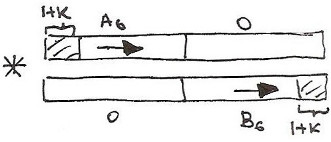
\includegraphics[width=5cm]{2.jpg}
\end{figure}\newline
\begin{figure}[hr]
	\includegraphics[width=5cm]{3.jpg}
\end{figure}\newline
\end{enumerate}
\end{enumerate}
\end{document}